\chapter{Projekt aplikacji}

\section{Wymagania funkcjonalne}

\subsection{Tworzenie grafów}
Podstawowym i oczywistym wymaganiem jest, aby użytkownik mógł stworzyć nowy, pusty graf skierowany oraz nieskierowany. Ponadto użytkownik powinien mieć możliwość zaimportowania istniejącego grafu oraz wygenerowania znanego grafu, np. cyklu lub grafu pełnego o zadanej ilości wierzchołków. 

\subsubsection{Importowanie grafów} \label{subsubsec:import}
Użytkownik powinien móc wczytać graf z komputera lub z chmury (np. Google Drive lub Dropbox) w trzech znanych formatach: 

\begin{itemize}
\setlength\itemsep{0em}
\item \texttt{GraphML},
\item \texttt{GEXF},
\item \texttt{JGF}.
\end{itemize}

Opisy formatów znajdują się w sekcji \ref{sec:graph-formats}.

\subsubsection{Generowanie grafów}

Użytkownik powinien mieć możliwość wygenerowania znanych grafów, dla zadanych parametrów wejściowych:

\begin{itemize}
\setlength\itemsep{0em}
\item grafu pustego,
\item grafu liniowego,
\item grafu cyklicznego,
\item koła,
\item grafu pełnego (lub turnieju dla grafów skierowanych),
\item grafu pełnego dwudzielnego,
\item grafu Petersena,
\item drzewa (o zadanej wysokości i ilości dzieci)
\end{itemize}

Definicje i przykłady powyższych grafów znajdują się w sekcji \ref{sec:common-graphs}.

Ponadto przydatnym dodatkiem w aplikacji będzie możliwość wygenerowania grafu losowego -- o danej ilości wierzchołków oraz parametrem prawdopodobieństwa określającym, czy pomiędzy dwoma wierzchołkami istnieje krawędź.  

\subsection{Wizualizacja}

Użytkownik powinien móc przesuwać widok, przybliżać i oddalać graf oraz rozmieszczać wierzchołki grafu w dowolny sposób. W aplikacji powinna istnieć możliwość zmiany układu grafu: układ oparty na oddziaływaniach (ang. \textit{force-based layout}), układ siatki, układ okręgu, układ koncentryczny, układ hierarchiczny. 

Użytkownik powinien być w stanie zmienić kategorię wierzchołka oraz typ krawędzi. Inne typy i kategorie powinny być oznaczone innym kolorem oraz powinna istnieć możliwość zmiany koloru. 

Aplikacja powinna również dostarczać opcję wyszukiwania i filtrowania danych (np. tylko dany typ wierzchołków, wierzchołki o stopniu większym niż zadany parametr). Przydatną funkcjonalnością będzie wyświetlanie sąsiadów danego wierzchołka po najechaniu na niego kursorem myszy.

\subsection{Edycja}

W aplikacji powinien istnieć osobny tryb edycji. Gdy użytkownik jest w tym trybie, powinien móc dodawać oraz usuwać wierzchołki i krawędzie. Powinien być w stanie także dodawać oraz modyfikować etykiety wierzchołków i krawędzi.

Użytkownik powinien mieć możliwość zaznaczania wielu wierzchołków i krawędzi na raz. Użyteczną funkcjonalnością będzie również grupowanie (lub rozgrupowanie) zaznaczonych wierzchołków. 

Aplikacja powinna wyświetlać ostatnio wykonaną akcję oraz udostępniać możliwość jej cofnięcia.

\subsection{Przetwarzanie}

Aplikacja powinna dawać możliwość wykonania podstawowych algorytmów na danym grafie:

\begin{itemize}
\setlength\itemsep{0em}
\item wyszukiwanie najkrótszej ścieżki pomiędzy dwoma wybranymi wierzchołkami,
\item znajdowanie minimalnego drzewa rozpinającego,
\item obliczanie algorytmu PageRank,
\item znajdowanie (silnie) spójnych składowych oraz dwuspójnych składowych,
\item znajdowanie cyklu Eulera,
\item znajdowanie cyklu Hamiltona.
\end{itemize}

\subsection{Eksportowanie}
Użytkownik powinien mieć możliwość wyeksportowania do formatów, które zostały przedstawione w podsekcji \ref{subsubsec:import}. 

Ponadto przydatną funkcjonalnością będzie możliwość wyeksportowania obecnego widoku do pliku graficznego, np. \texttt{PNG} lub \texttt{JPG}. 

\subsection{Udostępnianie grafu}
W aplikacji powinna istnieć możliwość udostępniania grafu innym użytkownikom. Po wybraniu tej opcji, powinien zostać wygenerowany unikalny odnośnik do grafu. Po przejściu na ten adres (w podstawowej wersji) inni użytkownicy mogą wyświetlić i edytować graf.



\section{Prototyp interfejsu użytkownika}

\begin{figure}[H]
\centering
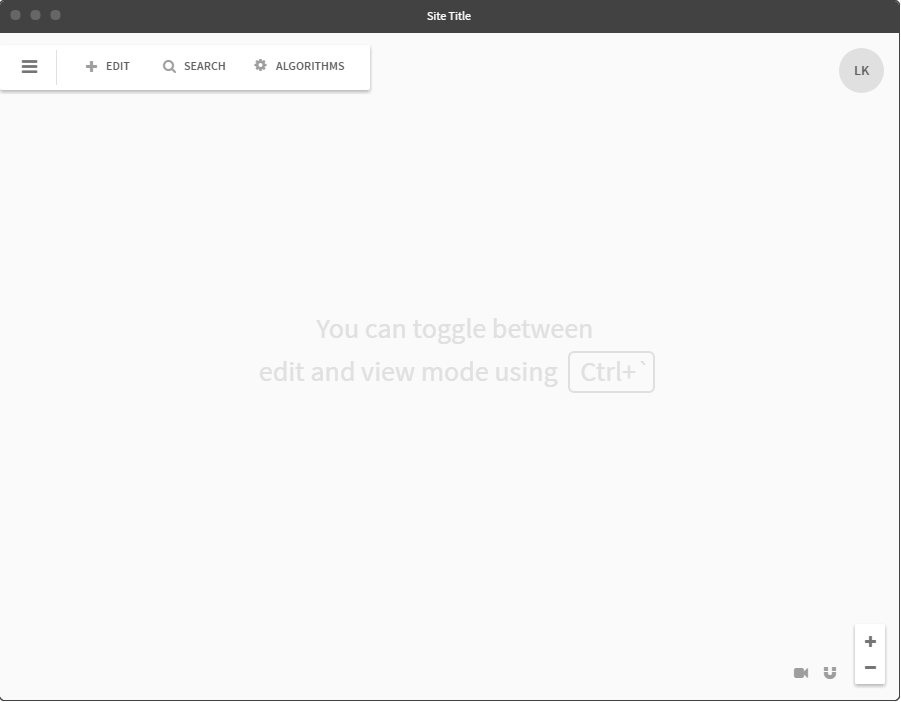
\includegraphics[width=\textwidth]{mock-view.png}
\caption{Tryb widoku grafu}
\end{figure}

\begin{figure}[H]
\centering
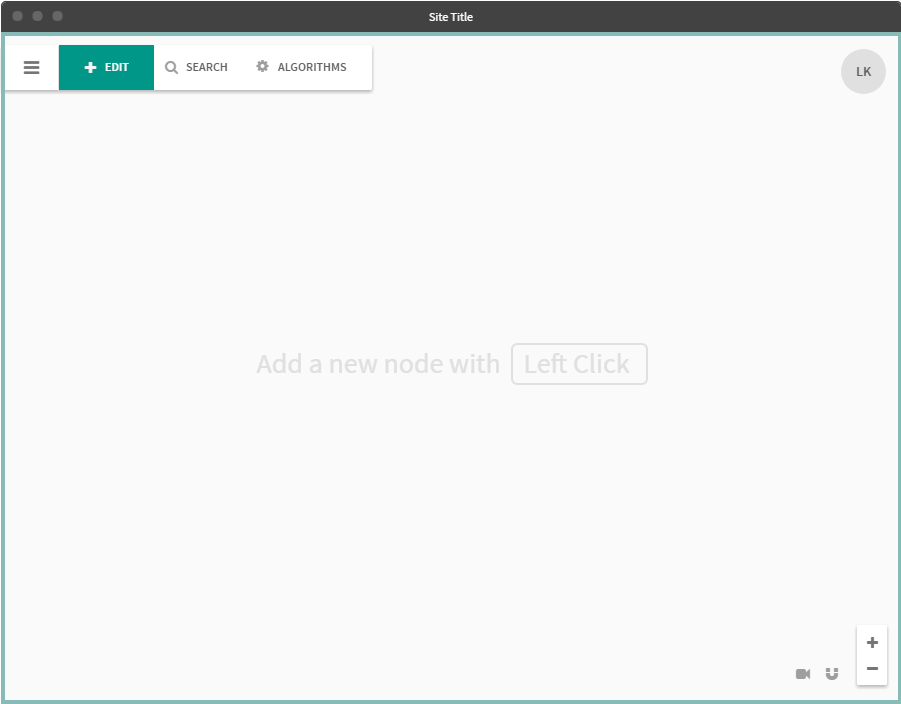
\includegraphics[width=\textwidth]{mock-edit.png}
\caption{Tryb edycji grafu}
\end{figure}

\begin{figure}[H]
\centering
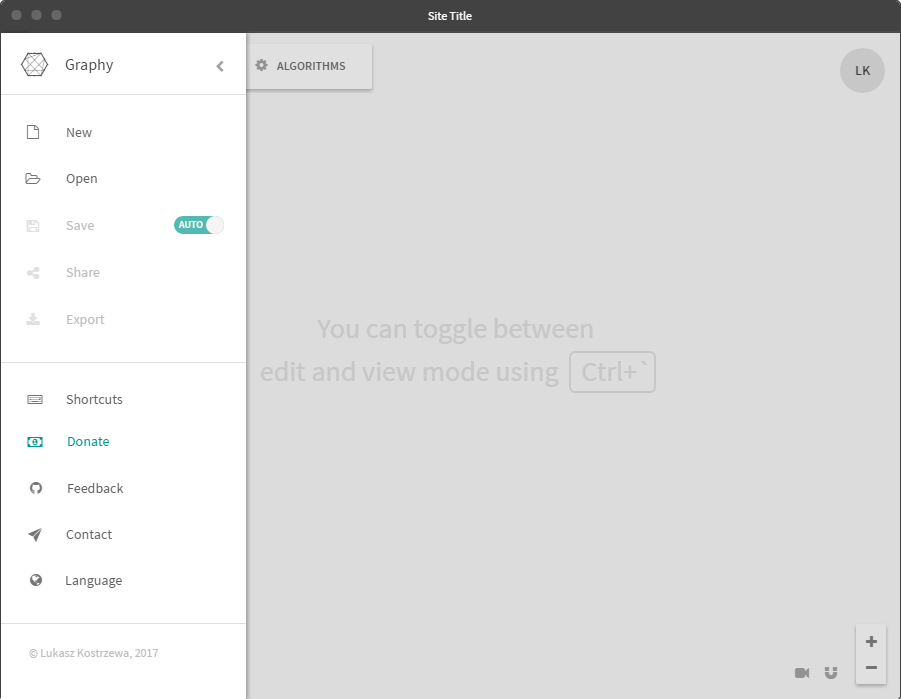
\includegraphics[width=\textwidth]{mock-menu.png}
\caption{Widok menu}
\end{figure}

\begin{figure}[H]
\centering
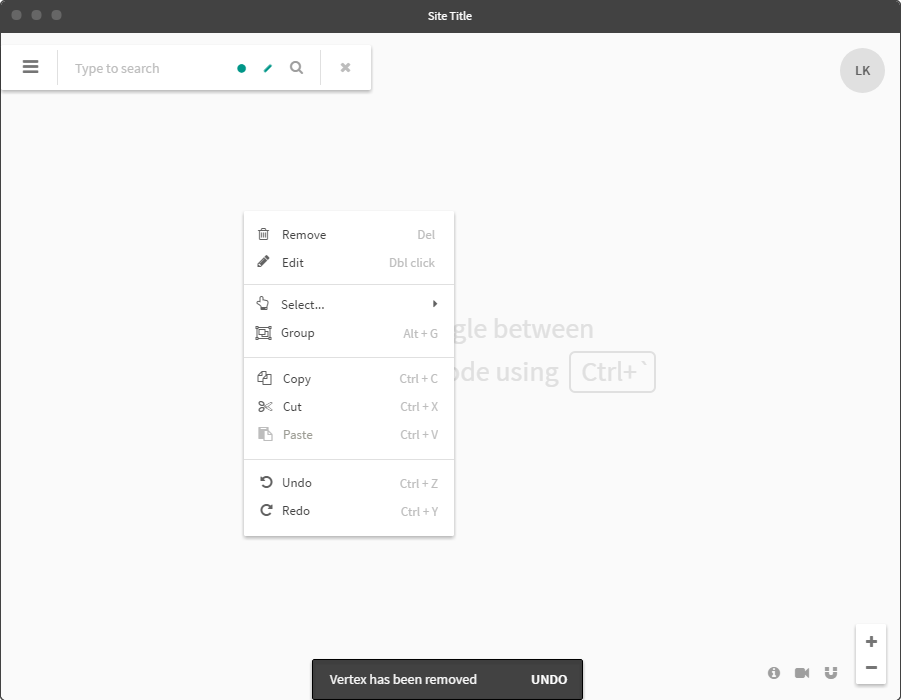
\includegraphics[width=\textwidth]{mock-context-menu.png}
\caption{Menu kontekstowe i informacja o ostatniej akcji}
\end{figure}